\documentclass{article}
\usepackage[utf8]{inputenc}
\usepackage{geometry}
\geometry{
    a4paper,
    total={170mm,257mm},
    left=20mm,
    top=20mm,
}
\usepackage{graphicx}
\usepackage{titling}
\usepackage{amsmath}
\usepackage{amsthm}
\usepackage{amssymb}
\usepackage{listings, listingsutf8}
\usepackage{xcolor}
\usepackage{hyperref}
\usepackage{tcolorbox}
\usepackage{enumitem}
\usepackage{booktabs} % For better looking tables
\usepackage{float}
\usepackage{lipsum}
\usepackage{cmbright}
\usepackage{todonotes}
\usepackage{minted}

\usemintedstyle{friendly}

\tcbset{
  defaultstyle/.style={
    colback=gray!10!white,
    colframe=gray!120,
    % fonttitle=\bfseries
  }
}

% Define theorem styles
\theoremstyle{plain} % Default style is italicized text
\newtheorem{theorem}{Theorem} % Number by section
\newtheorem{lemma}[theorem]{Lemma}
\newtheorem{proposition}[theorem]{Proposition}
\newtheorem{corollary}[theorem]{Corollary}


% Title and Author Information
\title{Karger\textquotesingle{}s Algorithm for Minimum Cut Problem}
\author{Charels Hugo}
\date{\today}

% Custom header and footer
\usepackage{fancyhdr}
\fancypagestyle{plain}{
    \fancyhf{} % clear all header and footer fields
    \fancyfoot[R]{
\includegraphics[width=2cm]{assets/pictures/ULB.png}}
    \fancyfoot[L]{\today}
    \fancyhead[L]{Asssignment 2}
    \fancyhead[R]{Charels Hugo}
}
% Header and Footer Customization
\pagestyle{fancy}
\fancyhf{}
\fancyfoot[L]{\today}
\fancyfoot[R]{
\includegraphics[width=2cm]{assets/pictures/ULB.png}}
\fancyhead[L]{INFO-F413}
\fancyhead[R]{Charels Hugo}


\makeatletter
\def\@maketitle{%
  \newpage
  \null
  \vskip 1em%
  \begin{center}%
  \let \footnote \thanks
    {\LARGE \@title \par}%
    \vskip 1em%
    % {\large \@date}%
  \end{center}%
  \par
  \vskip 1em}
\makeatother

\begin{document}

\maketitle

\noindent\begin{tabular}{@{}ll}
    Students     & Charels Hugo \\
    Course       & INFO-F413 \\
    Instructors  & Jean Cardinal \\
\end{tabular}


\begin{abstract}
This report explores Karger\textquotesingle{}s algorithms for the minimum cut problem, focusing on the Contract and FastCut variations. Implementations are presented, success probabilities evaluated under constrained time budgets, and theoretical results verified through experiments. Complete and planar graphs are analyzed due to their contrasting topological properties and importance in graph algorithm studies. Experimental findings confirm theoretical predictions and provide insights into algorithm performance and efficiency.
\end{abstract}


\section{Introduction}
The minimum cut problem involves partitioning the vertex set of a graph $G = (V, E)$ into two non-empty subsets such that the number of edges crossing the subsets is minimized. Karger\textquotesingle{}s randomized contraction algorithm offers an innovative probabilistic solution, combining simplicity with strong theoretical guarantees.

This study focuses on implementing and comparing the Contract and FastCut algorithms, with particular attention to verifying the following theorem:
\begin{theorem}[FastCut Success Probability]
The FastCut algorithm succeeds in finding a minimum cut with probability $\Omega(1/\log n)$.
\end{theorem}

Complete and planar graphs are chosen as test cases due to their theoretical and practical significance. Complete graphs, characterized by maximum edge density, provide a challenging scenario for edge-based algorithms, while planar graphs, constrained by structural properties, often exhibit unique algorithmic behavior. By examining these graph families, we aim to connect theoretical insights with empirical performance.


\section{Algorithm Description}

\subsection{The Contract Algorithm}
The Contract algorithm iteratively contracts randomly chosen edges until only two vertices remain. The resulting cut corresponds to the partition of these vertices. The algorithm\textquotesingle{}s success probability is at least $\frac{2}{n(n-1)}$ for an input graph with $n$ vertices. 

\paragraph{Implementation} The algorithm is implemented in Rust (see Appendix \ref{appendix:contract}).

\subsection{The FastCut Algorithm}
FastCut enhances the Contract algorithm by recursively applying it to smaller subgraphs. The steps are as follows:
\begin{enumerate}
    \item If $n \leq 6$, compute the minimum cut via brute force.
    \item Otherwise, set $t = \lceil 1 + n/\sqrt{2} \rceil$.
    \item Perform two independent Contract algorithm until $t$ vertices remain, yielding subgraphs $H_1$ and $H_2$.
    \item Recursively compute the minimum cuts of $H_1$ and $H_2$.
    \item Return the smaller of the two cuts.
\end{enumerate}

FastCut improves the success probability to $\Omega(1/\log n)$ while maintaining a runtime complexity of $O(n^2 \log n)$.

\paragraph{Implementation} The algorithm is implemented in Rust (see Appendix \ref{appendix:fast_cut}).


\section{Experimental Plan}
Our experiments focus on complete and planar graphs to evaluate the performance of Karger\textquotesingle{}s algorithms. For planar graphs, instances were constructed with the maximum number of edges, $|E| = 3|V| - 6$, as dictated by Euler\textquotesingle{}s formula, ensuring challenging test cases.

The experimental goals are:
\begin{enumerate}
    \item Verify theoretical success probability bounds:
    \begin{enumerate}
        \item Run each algorithm 100 times on graphs of varying sizes.
        \item Compare observed success rates with theoretical bounds.
    \end{enumerate}
    \item Compare performance under equal time constraints:
    \begin{enumerate}
        \item Measure the runtime of a single FastCut execution.
        \item Run Contract repeatedly within the same time frame.
        \item Compare the success rates of both approaches.
    \end{enumerate}
\end{enumerate}

Metrics include success probability, runtime, and the impact of graph topology on performance. Each experiment is repeated 100 times for statistical robustness.


\section{Experimental Results}

\subsection{Verification of Probability Bounds}

For complete graphs, FastCut consistently achieved a 100\% success rate, while the Contract algorithm demonstrated slightly lower probabilities, as shown in Figure \ref{fig:complete-success-bounds}.

\begin{figure}[H]
    \centering
    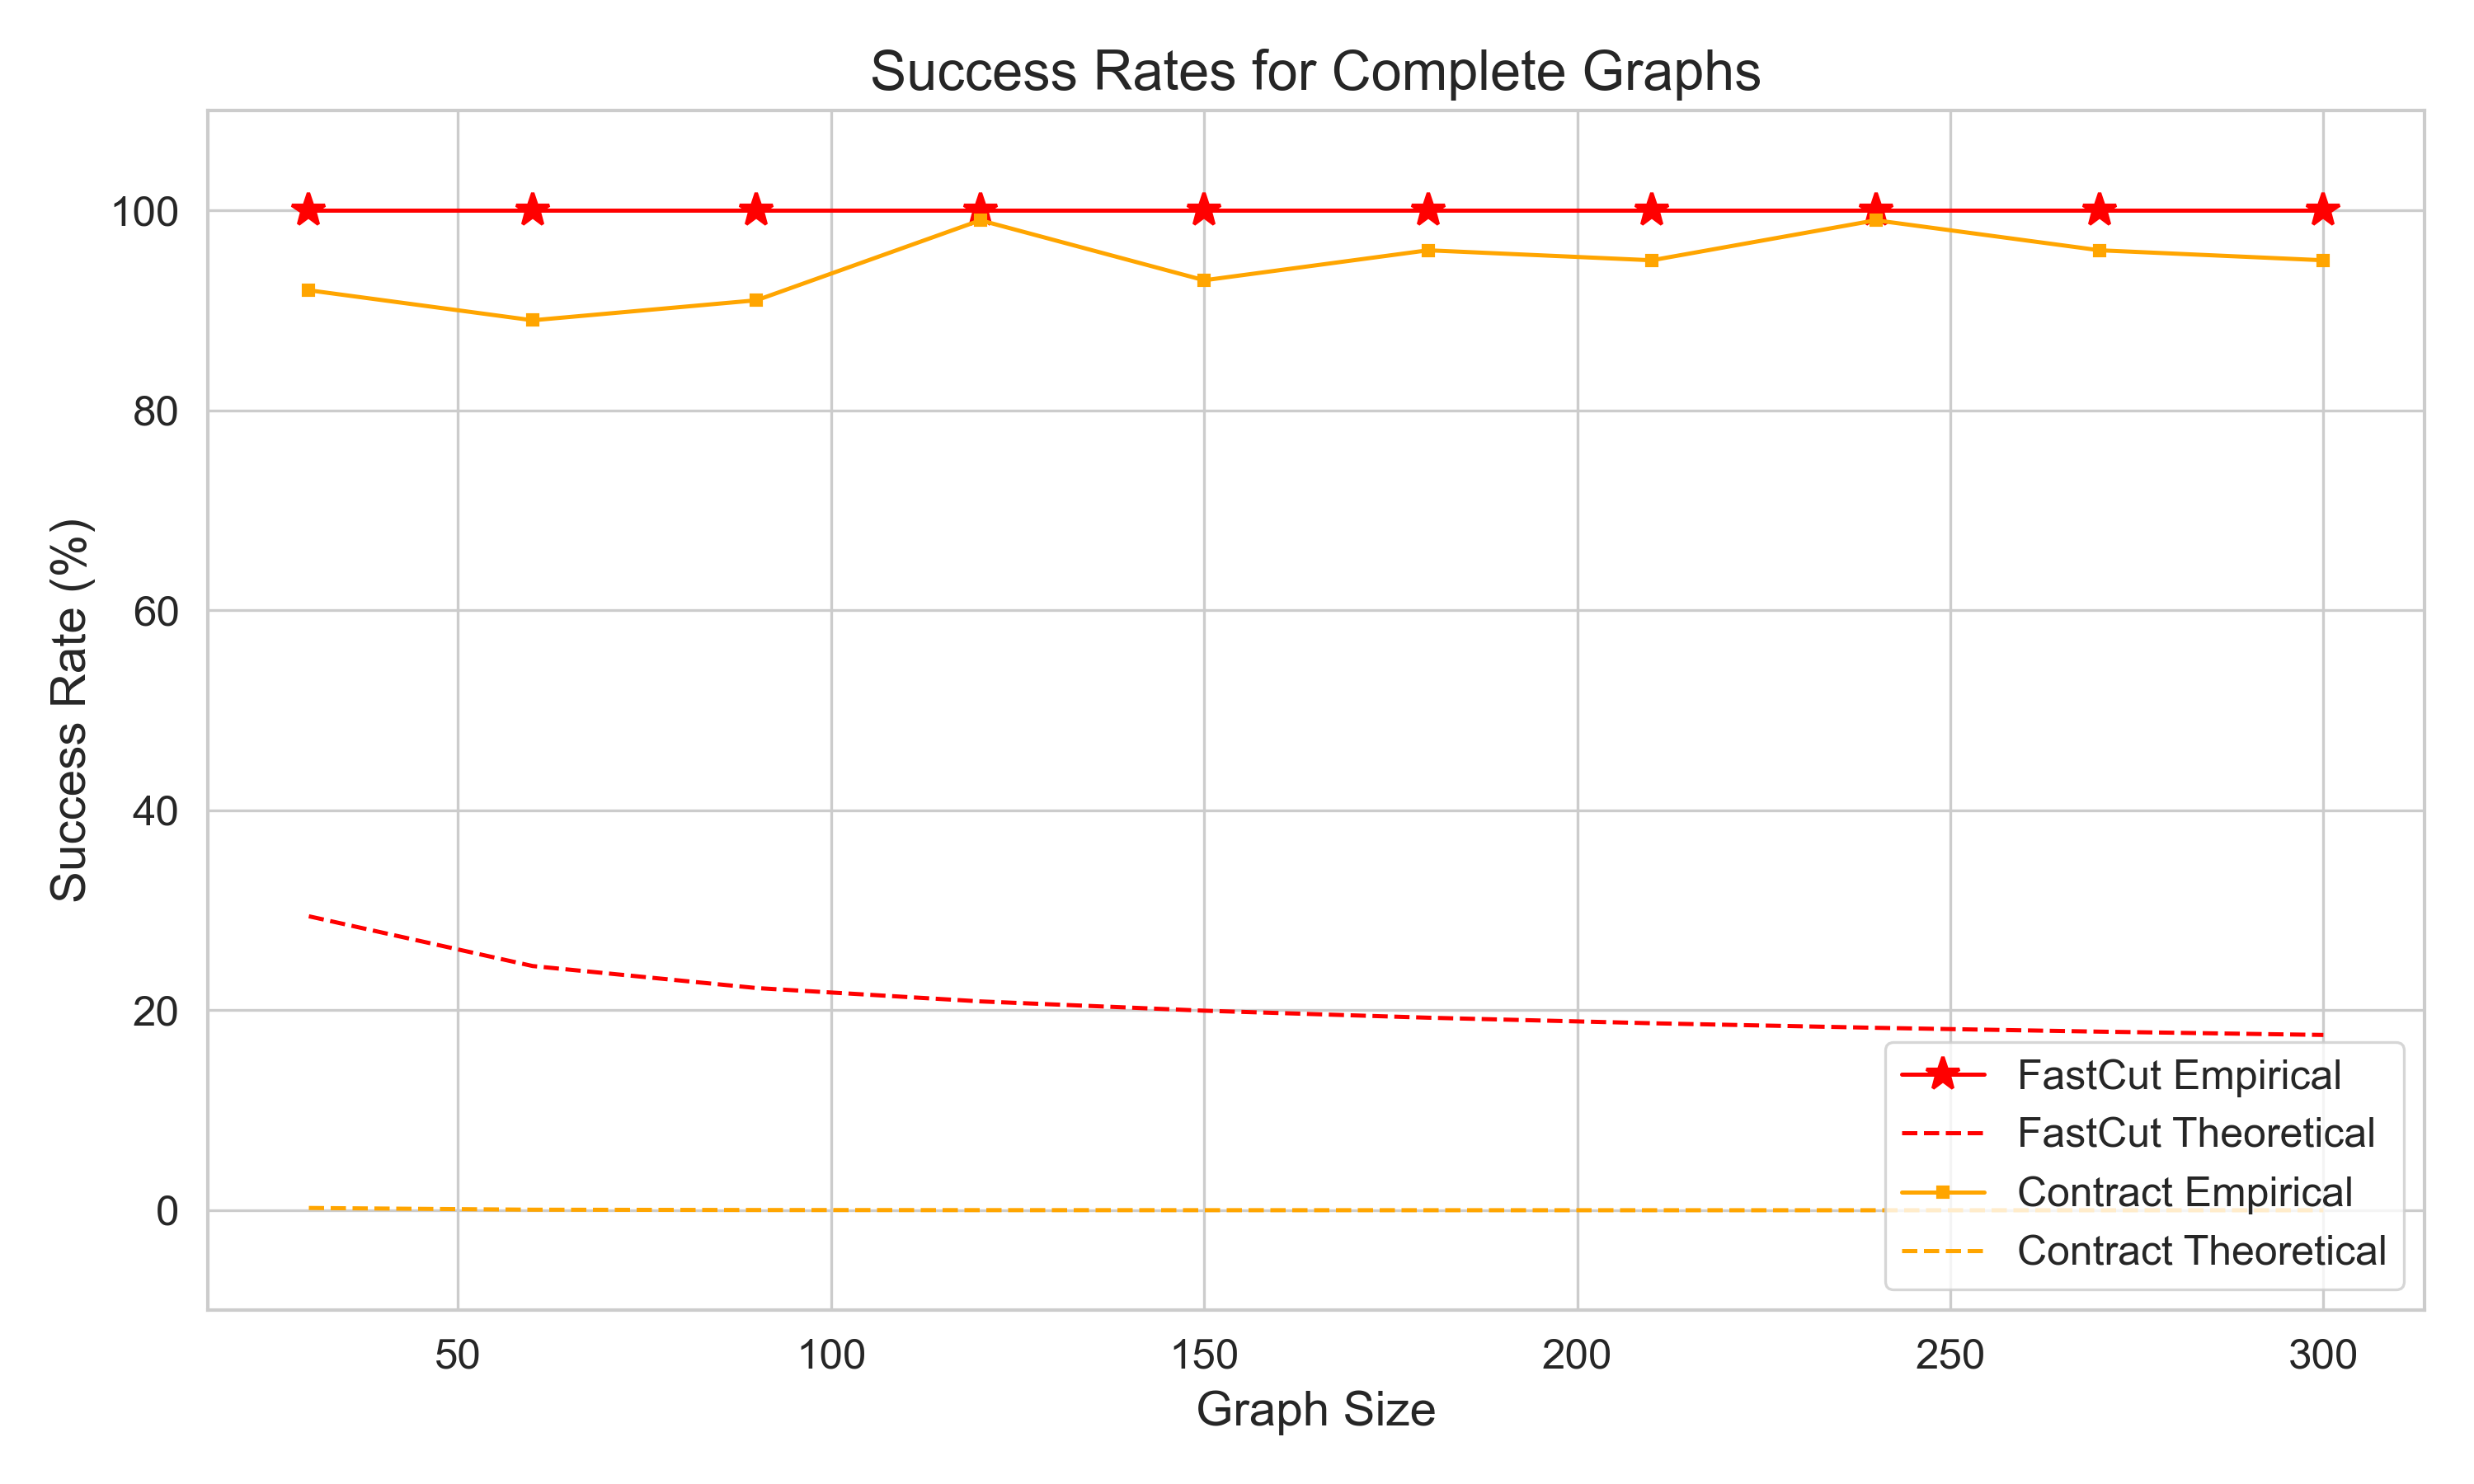
\includegraphics[width=0.8\linewidth]{assets2//graphics/success_bounds_300_complete_success_plot.png}
    \caption{Success probability of FastCut and Contract algorithms on complete graphs.}
    \label{fig:complete-success-bounds}
\end{figure}

For planar graphs, FastCut maintained near-perfect performance, with success rates close to 100\% in all trials. In contrast, Contract often fell below 40\%, as depicted in Figure \ref{fig:planar-success-bounds}.

\begin{figure}[H]
    \centering
    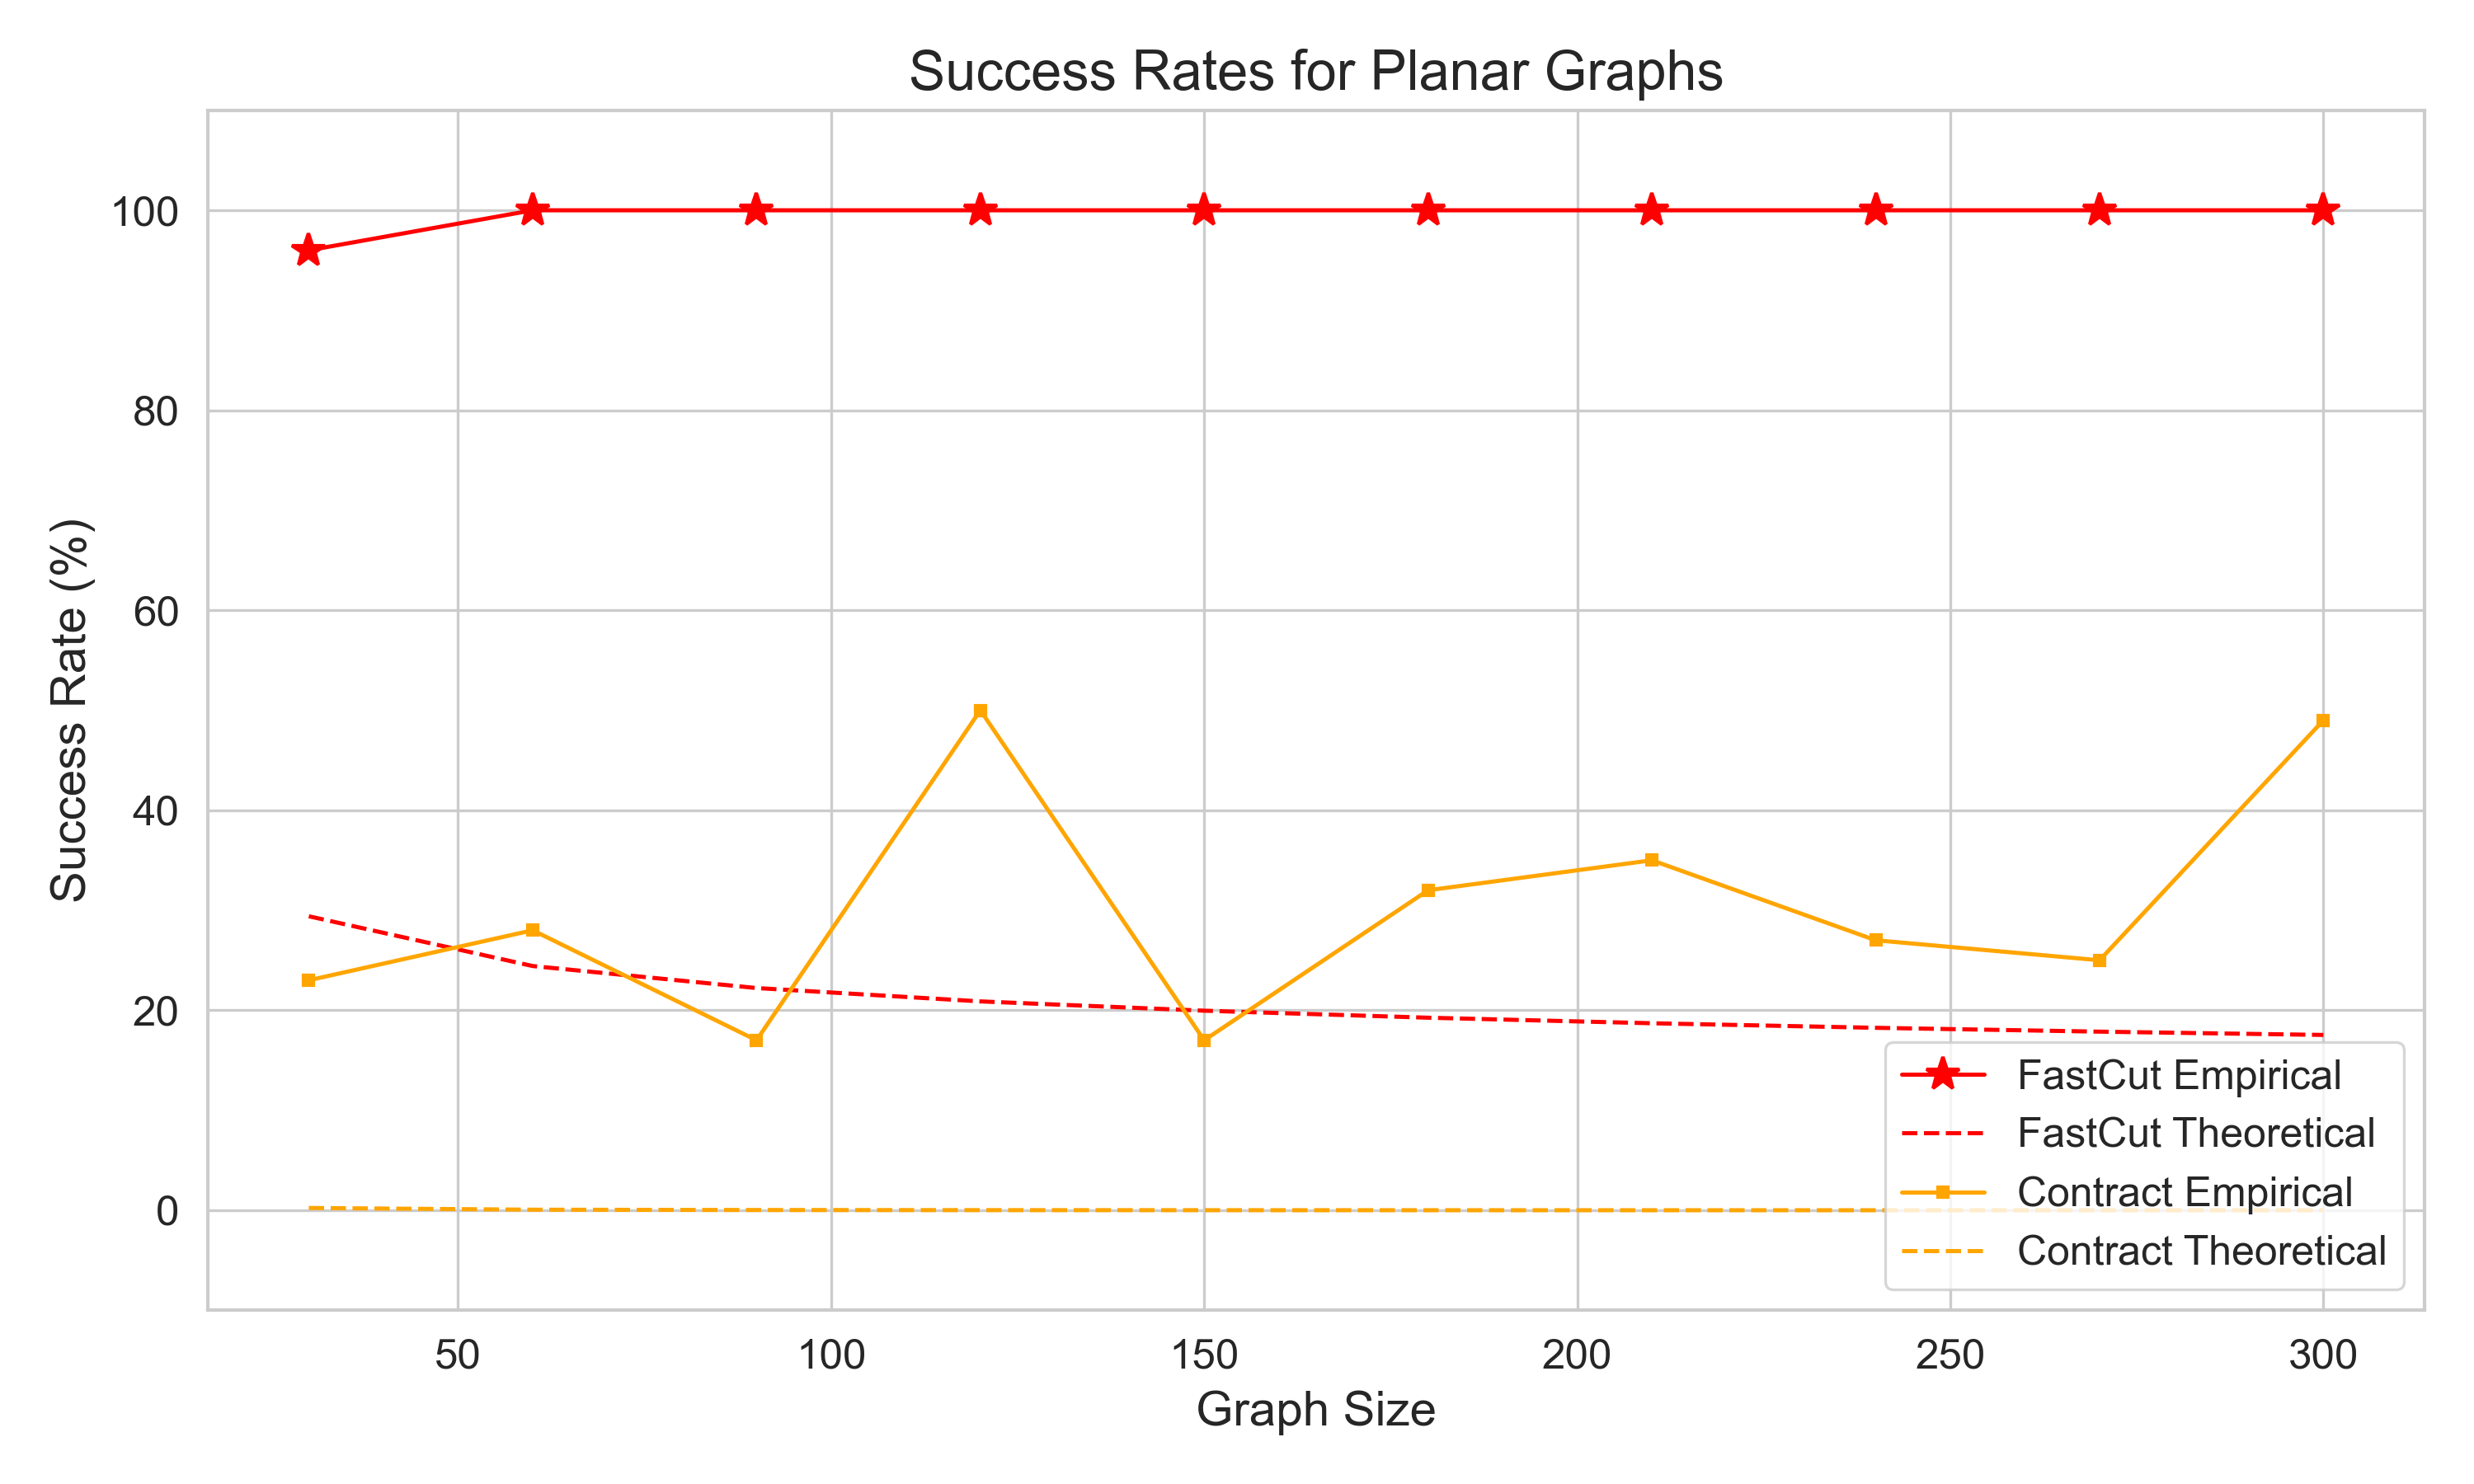
\includegraphics[width=0.8\linewidth]{assets2//graphics/success_bounds_300_planar_success_plot.png}
    \caption{Success probability of FastCut and Contract algorithms on planar graphs.}
    \label{fig:planar-success-bounds}
\end{figure}

\subsection{Performance Under Equal Time Constraints}
Under identical time budgets, FastCut achieved a 100\% success rate on complete graphs in a single run, while Contract required multiple runs to reach comparable rates (Figure \ref{fig:complete-same-time}).

\begin{figure}[H]
    \centering
    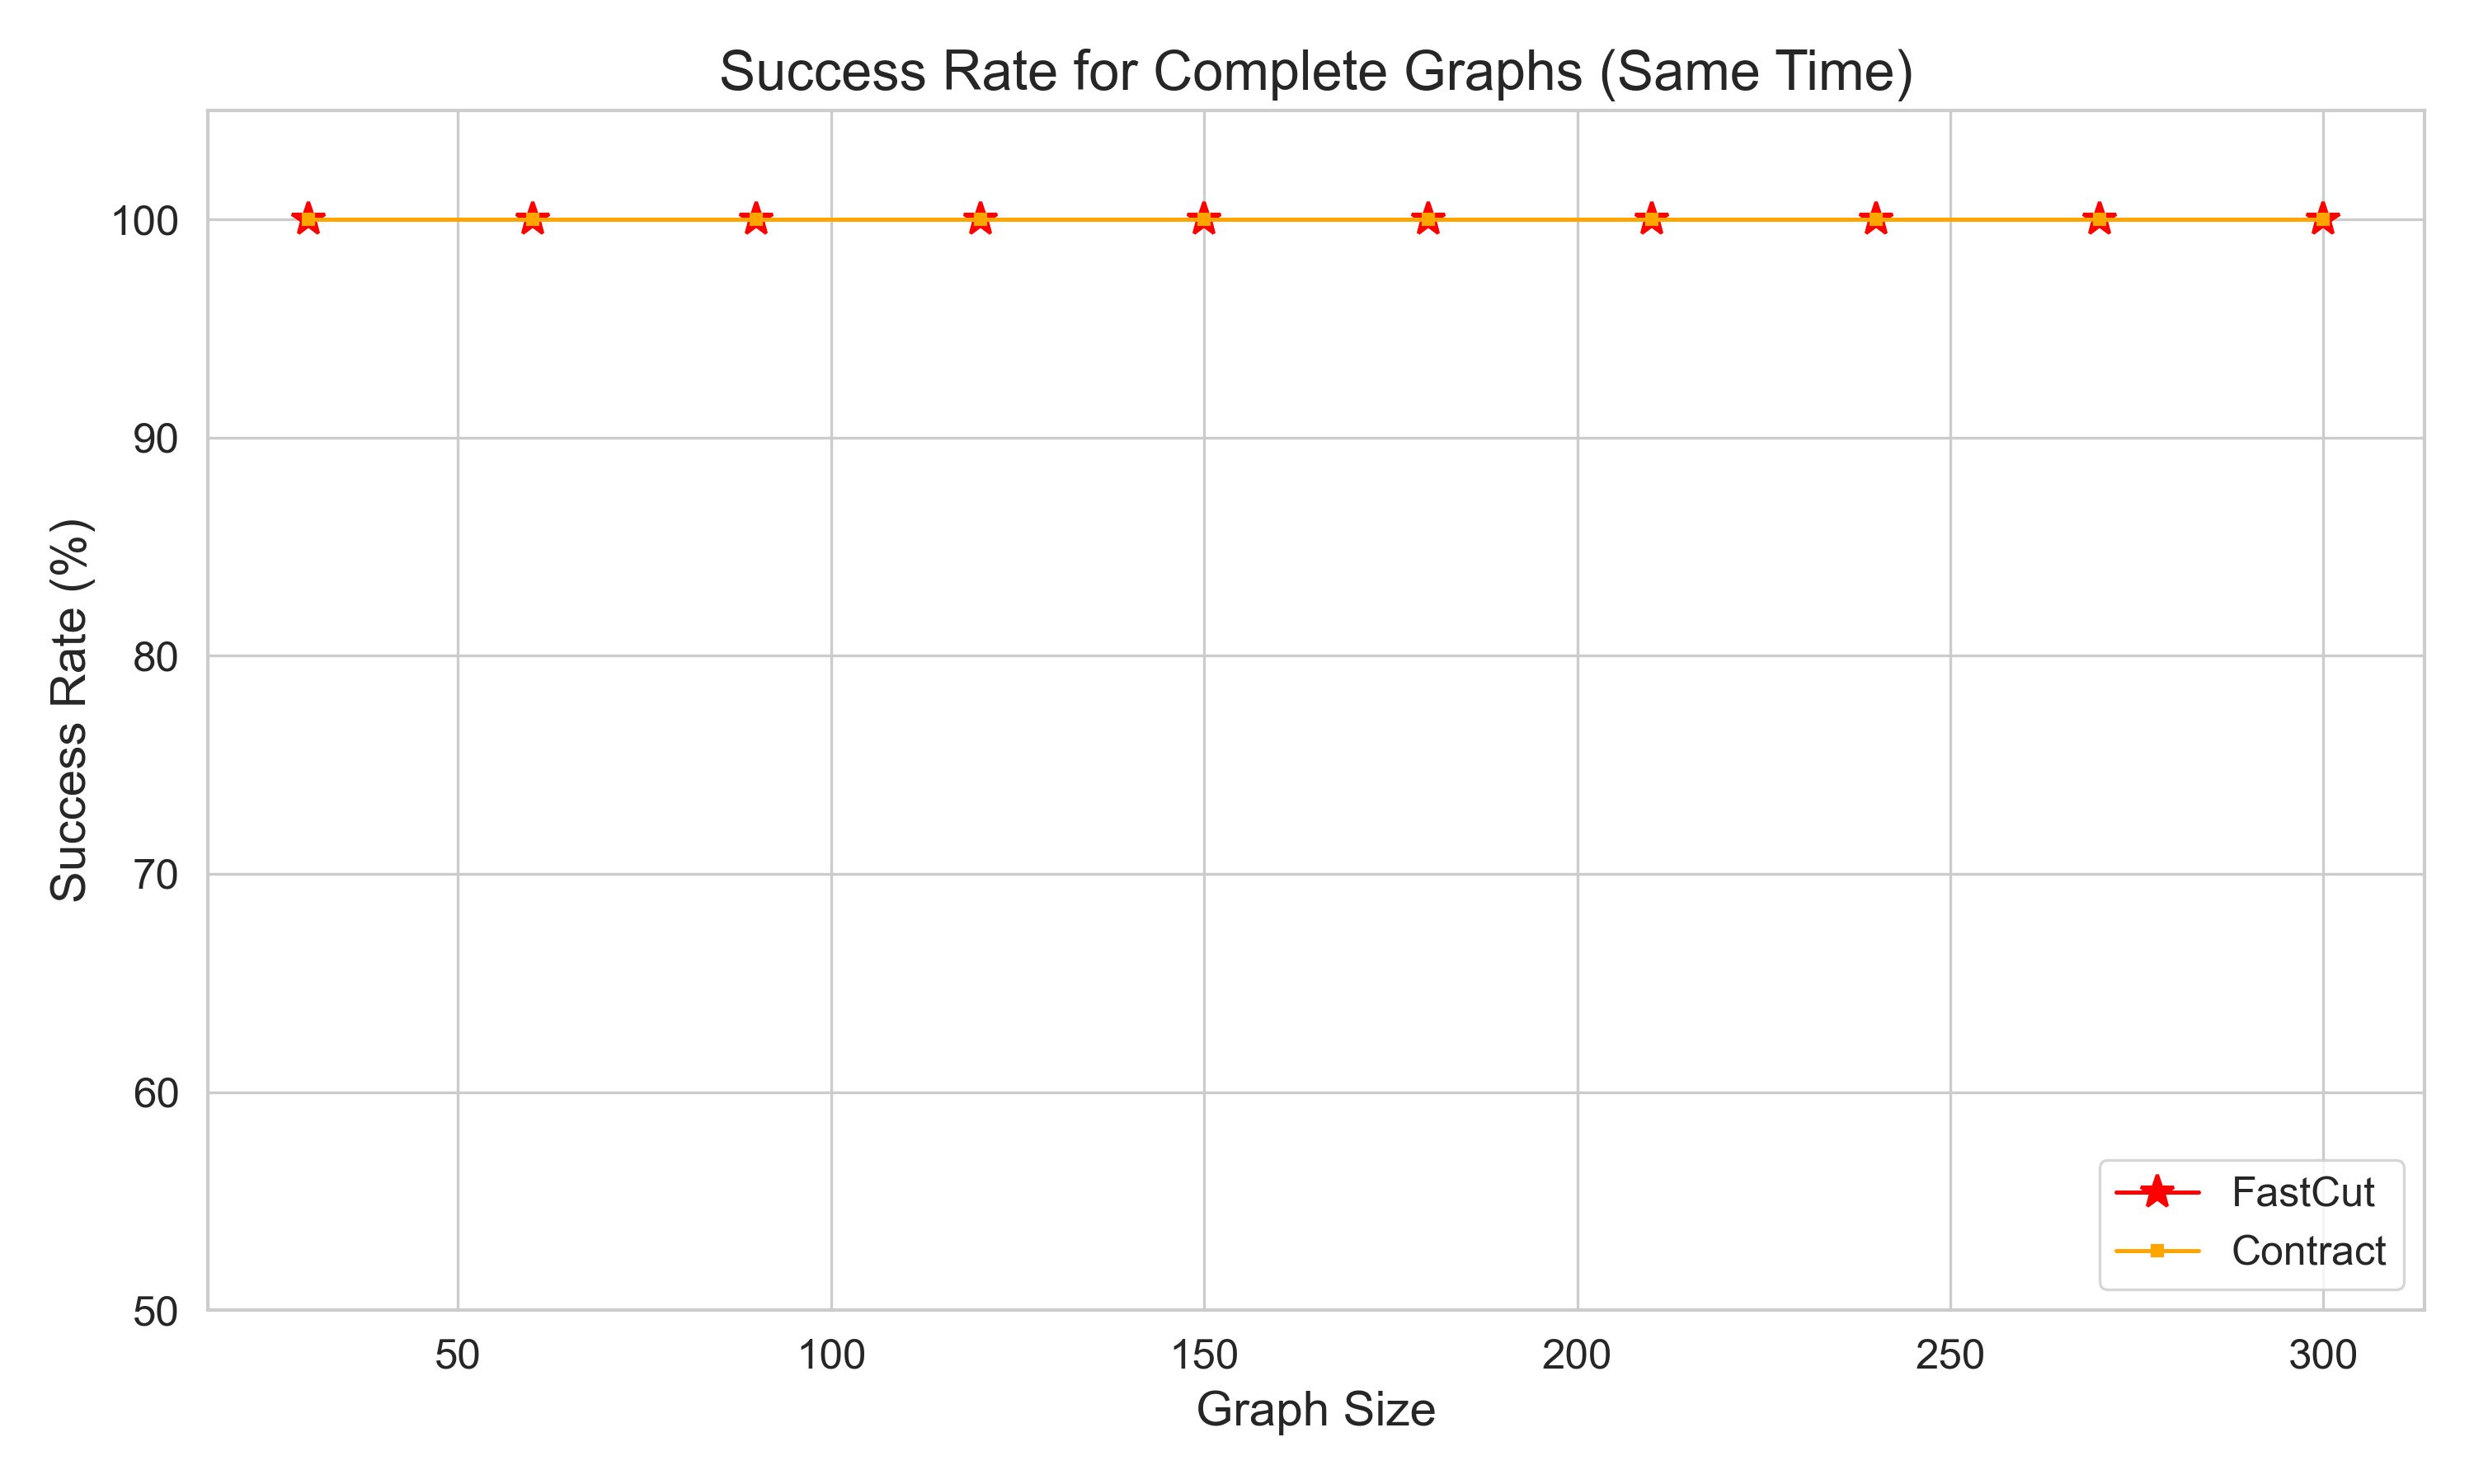
\includegraphics[width=0.8\linewidth]{assets2//graphics/same_time_300_complete_same_time_plot.png}
    \caption{Comparison of success rates for FastCut and Contract on complete graphs under equal time constraints.}
    \label{fig:complete-same-time}
\end{figure}

For planar graphs, Contract consistently achieved 100\% success rates, while FastCut remained above 90\% (Figure \ref{fig:planar-same-time}).

\begin{figure}[H]
    \centering
    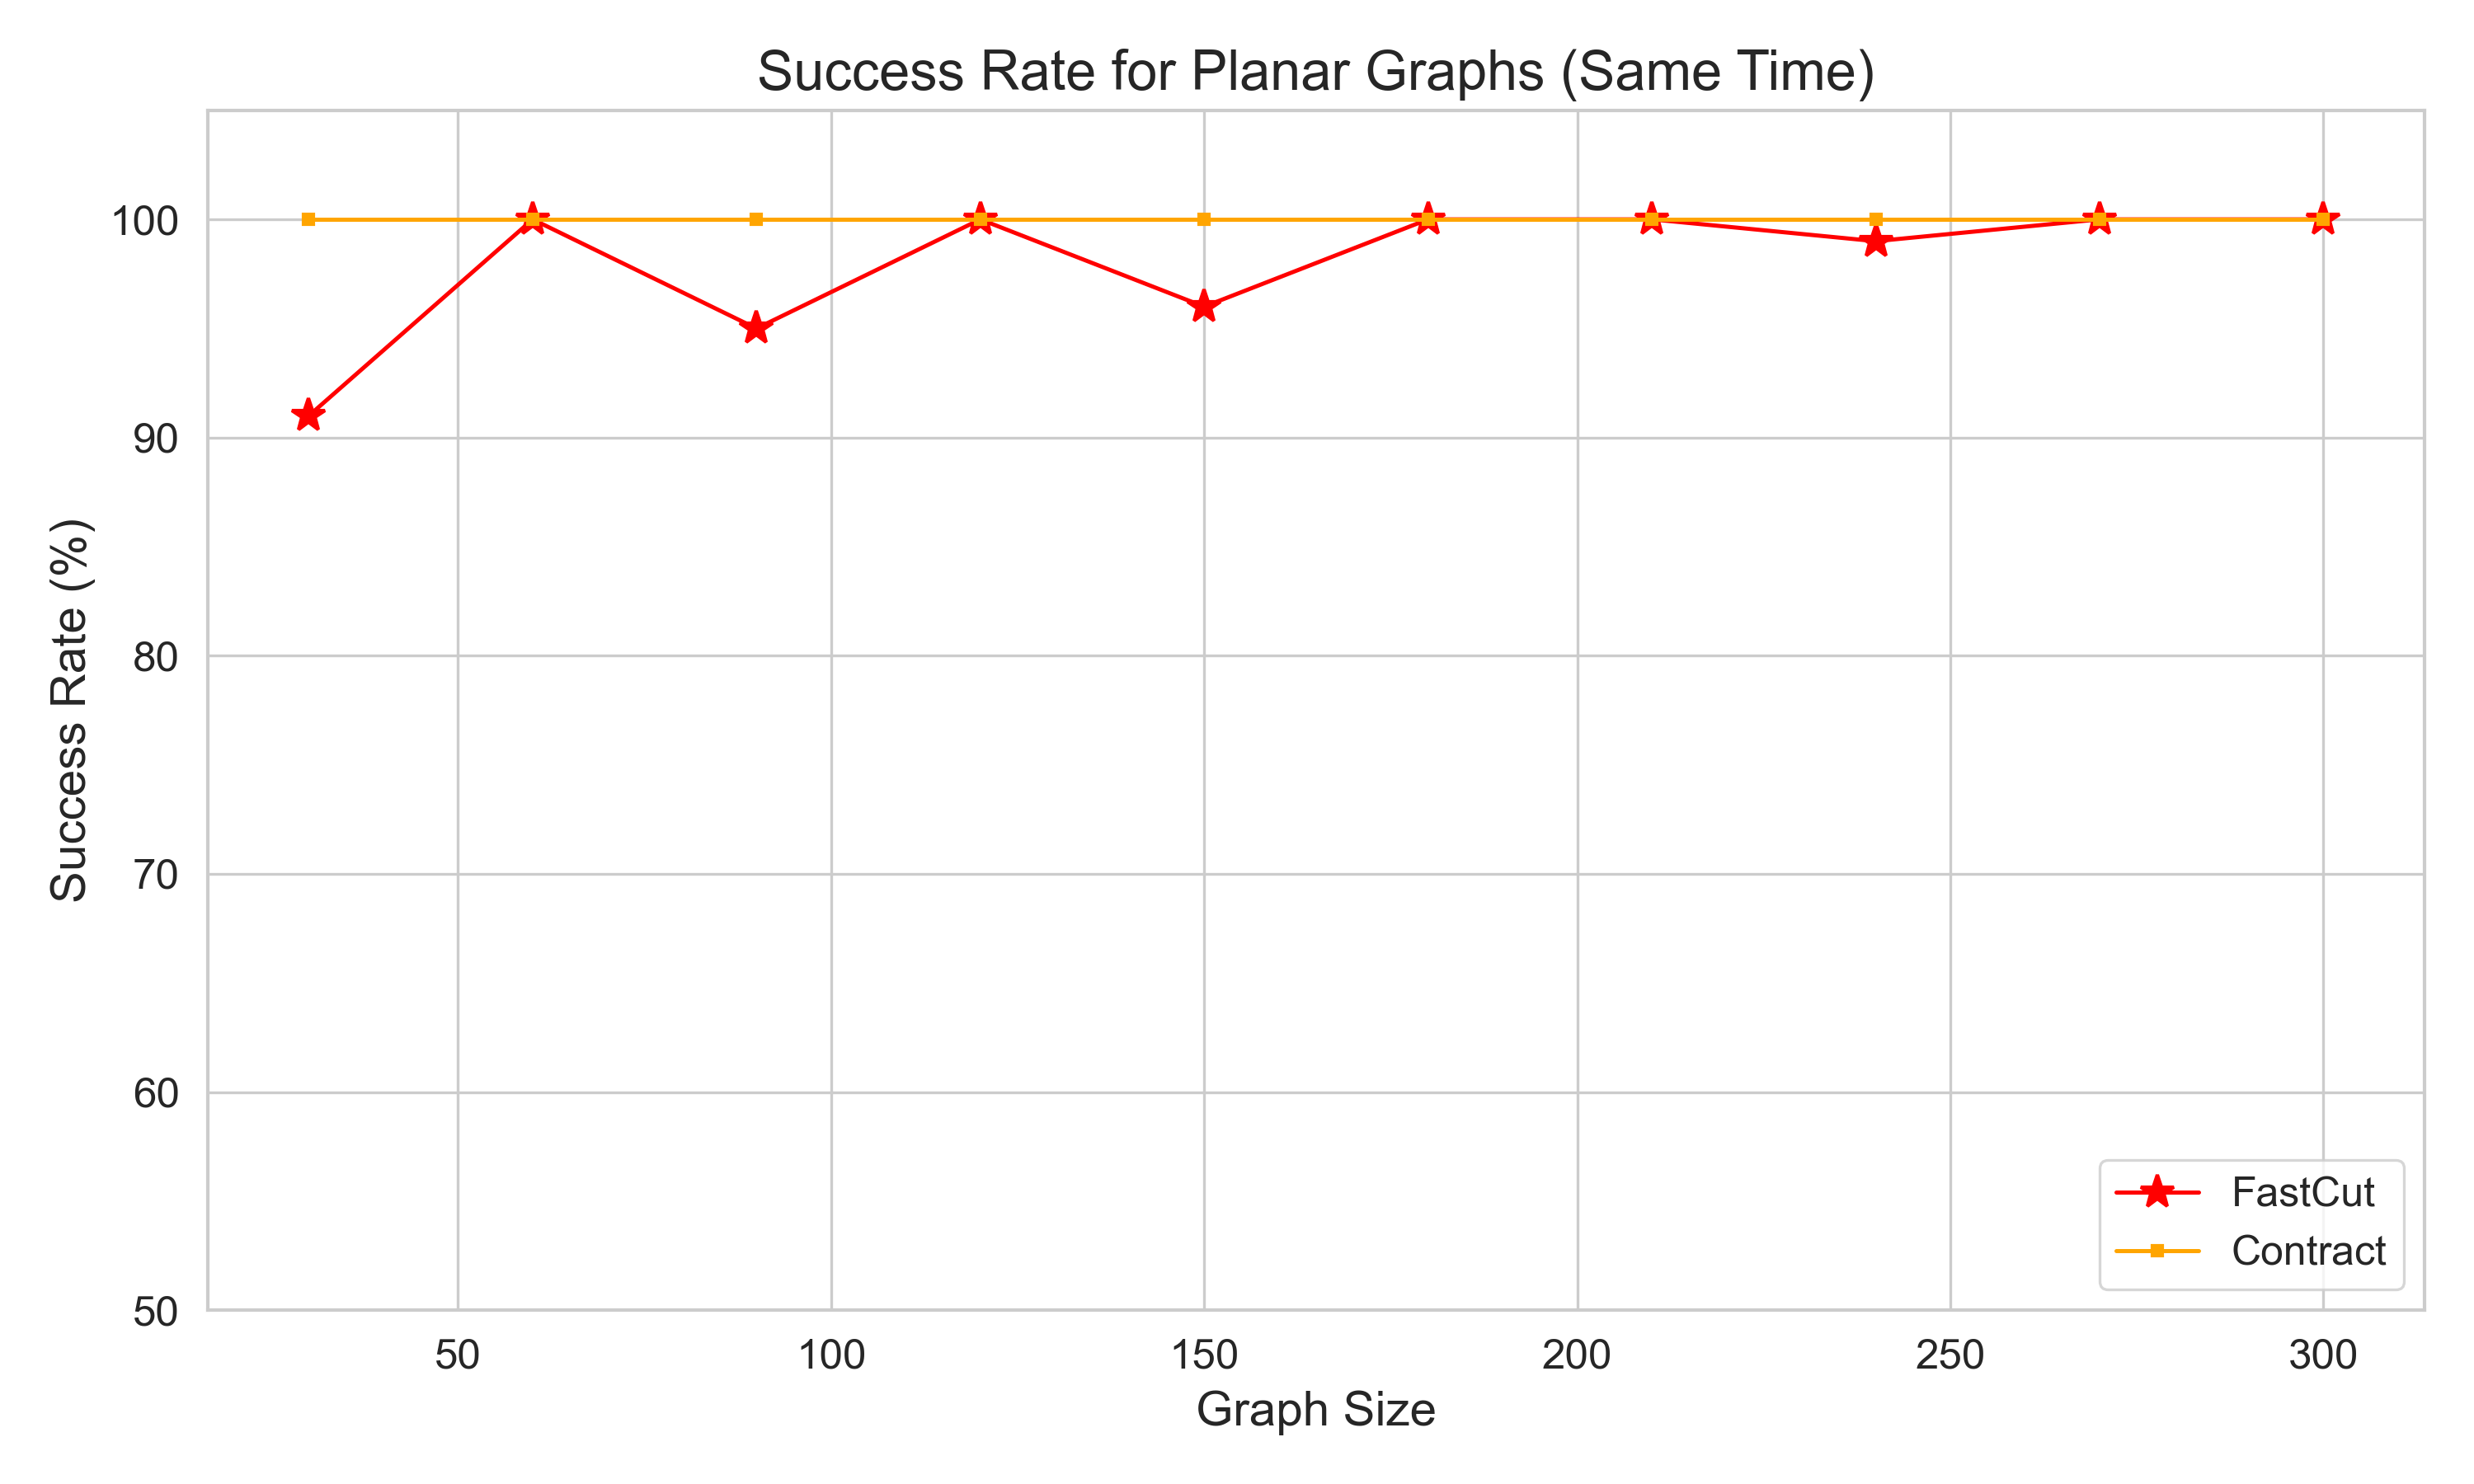
\includegraphics[width=0.8\linewidth]{assets2//graphics/same_time_300_planar_same_time_plot.png}
    \caption{Comparison of success rates for FastCut and Contract on planar graphs under equal time constraints.}
    \label{fig:planar-same-time}
\end{figure}


\section{Discussion}
The higher success rate of the Contract algorithm on complete graphs can be attributed to their dense edge structure. With ${n \choose 2}$ edges, the likelihood of contracting a non-minimum cut edge is lower, enhancing the probability of preserving a minimum cut. Conversely, planar graphs, with their edge count limited by Euler\textquotesingle{}s formula, increase the risk of contracting a minimum cut edge, reducing success rates.

Comparisons under equal time constraints highlight the tradeoff between algorithm complexity and runtime efficiency. FastCut\textquotesingle{}s recursive nature ensures high single-run success probabilities but limits the number of runs possible within a fixed time. Repeated runs of Contract compensate for its lower single-run probability, achieving higher aggregate success rates.


\section{Conclusion}
This study evaluated Karger\textquotesingle{}s Contract and FastCut algorithms on complete and planar graphs, validating theoretical predictions with empirical data. Results demonstrate that Contract performs better on complete graphs due to their dense edge structure, while planar graphs pose challenges due to sparsity. FastCut, though slower, consistently achieves high success rates.

For future work, we propose extending this analysis to other graph classes, and experimenting with larger graph sizes. These directions could provide deeper insights into the scalability and adaptability of Karger's algorithms. Unfortunately, the scope of this study was limited by the computational resources and time available, which constrained the size and variety of graphs that could be tested.


\section*{Disclaimer}
This document was co-written with the assistance of generative AI, primarily for improving grammar, style, and clarity. The ideas, results, and analyses are the work of the authors.


\newpage

\appendix
\section{Source Code}
\label{appendix:code}

\subsection{Contract}
\label{appendix:contract}
\inputminted[
    linenos,          % Adds line numbers
    frame=lines,      % Adds a frame around the code
    framesep=5pt,     % Space between the frame and the code
    bgcolor=gray!5,  % Light gray background color
    fontsize=\small,  % Adjust font size if needed
]{rust}{assets2/code/contract.rs}

\subsection{FastCut}
\label{appendix:fast_cut}
\inputminted[
    linenos,          % Adds line numbers
    frame=lines,      % Adds a frame around the code
    framesep=5pt,     % Space between the frame and the code
    bgcolor=gray!5,  % Light gray background color
    fontsize=\small,  % Adjust font size if needed
]{rust}{assets2/code/fast_cut.rs}

\label{appendix:min_cut}
\inputminted[
    linenos,          % Adds line numbers
    frame=lines,      % Adds a frame around the code
    framesep=5pt,     % Space between the frame and the code
    bgcolor=gray!5,  % Light gray background color
    fontsize=\small,  % Adjust font size if needed
]{rust}{assets2/code/min_cut.rs}


\subsection{Graph}
\label{appendix:graph_interface}
\inputminted[
    linenos,          % Adds line numbers
    frame=lines,      % Adds a frame around the code
    framesep=5pt,     % Space between the frame and the code
    bgcolor=gray!5,  % Light gray background color
    fontsize=\small,  % Adjust font size if needed
]{rust}{assets2/code/graph_interface.rs}

\label{appendix:graph_impl}
\inputminted[
    linenos,          % Adds line numbers
    frame=lines,      % Adds a frame around the code
    framesep=5pt,     % Space between the frame and the code
    bgcolor=gray!5,  % Light gray background color
    fontsize=\small,  % Adjust font size if needed
]{rust}{assets2/code/graph_impl.rs}


\end{document}